%%%%%%%%%%%%%%%%%%%%%%%%%%%%%%%%%%%%%%%%%%%%%%%%%%%%%%%%%%%%%%%%%%%%%%%%%%%%%%%%
%2345678901234567890123456789012345678901234567890123456789012345678901234567890
%        1         2         3         4         5         6         7         8

\documentclass[conference]{ieeeconf}
%\usepackage{times}

% Subfiles package
%\usepackage{subfiles}

% References
%\usepackage[numbers]{natbib}

% Usual setup packages
\usepackage{listings} % For including source code with highlighting
\usepackage{hyperref} % For better hyper-link integration
\usepackage[bottom]{footmisc} % places footnotes at page bottom

% Packages for verbatim text blocks
\usepackage{alltt} % Package for including math in verbatim text
\usepackage{fancyvrb}

% Packages for math symbols and other mathey things
%\usepackage{amsthm}
\newtheorem{theorem}{Theorem}
\newtheorem{claim}{Claim}
\newtheorem{corollary}{Corollary}
\newtheorem{proposition}{Proposition}
\usepackage{amsmath}
\usepackage{amsfonts}
\usepackage{amssymb}

% Packages for including pseudo-code
\usepackage{algorithmicx}
\usepackage{algorithm}
\usepackage{algpseudocode}

% Packages that handle tables, figures and other floats
\usepackage{enumerate}
\usepackage{tabularx}
\usepackage{multirow}
\usepackage{float} % To make floats movable
\usepackage{subcaption}
\usepackage[table]{xcolor}

% Packages for drawing graphs, FSMs, etc.
\usepackage{pgf}
\usepackage{tikz}
\usetikzlibrary{shapes,arrows,calc,fit,positioning,shapes.symbols,shapes.callouts,patterns,automata,matrix}

% Remove red boxes around refs
\hypersetup{
    colorlinks,
    citecolor=black,
    filecolor=black,
    linkcolor=black,
    urlcolor=blue
}

% ------------------------------ CUSTOM MACROS ------------------------------------
% Nice little macro for adding a comment box. Include incrementing comment numbers.
\newcounter{comcount}
\setcounter{comcount}{0}
\newcommand{\mycomment}[1]
{
\refstepcounter{comcount}
\smallskip\noindent\fbox{\parbox{\linewidth}{\emph{Comment \arabic{comcount}} : \small{#1}}} 
}

\DeclareMathOperator*{\argmin}{\arg\!\min\>}
\newcommand{\amin}[1]{\underset{#1}\argmin}
\DeclareMathOperator*{\argmax}{\arg\!\min\>}
\newcommand{\amax}[1]{\underset{#1}\argmax}

\def\a{\mathbf{a}}
\def\Z{\mathbb{Z}}
\def\R{\mathbb{R}}
\def\N{\mathcal{N}}
\def\estt{\hat{\tau}}
\def\estg{\gamma}
\newcommand{\sig}{\mathcal{S}}
\newcommand{\ceil}[1]{\lceil#1\rceil}
\newcommand{\xm}{x_{\hat{m}}}

\begin{document}
\title{Modeling Multi-Robot Task Assignment as a Global Game}

\author{\authorblockN{Anshul Kanakia and Nikolaus Correll}
\authorblockA{College of Engineering and Applied Sciences\\
Computer Science\\
University of Colorado, Boulder\\
Boulder -- Colorado, USA\\
Email: anshul.kanakia@colorado.edu\\
Email: nikolaus.correll@colorado.edu}
\and
\authorblockN{Behrouz Touri}
\authorblockA{College of Engineering and Applied Sciences\\
Electrical Engineering\\
University of Colorado, Boulder\\
Boulder -- Colorado, USA\\
Email: behrouz.touri@colorado.edu}}

\maketitle

%%%%%%%%%%%%%%%%%%%%%%%%%%%%%%%%%%%%%%%%%%%%%%%%%%%%%%%%%%%%%%%%%%%%%%%%%%%%%%%%
\begin{abstract}
We show that using an agent level threshold strategy for the task assignment problem in swarm robotics results in system level equilibrium for a certain class of collaborative tasks that have the property of \emph{concurrent benefit}. While threshold policies have long been used by swarm roboticists to model task assignment, the justification for their use has always been phenomenological in nature; drawing inspiration from threshold based task assignment models in biological systems such as ant colonies. We, instead, present a proof derived from the theory of global games to show that individual agent threshold response strategies for task assignment do indeed result in system-wide equilibrium (but not necessarily system-wide optimum), under certain conditions.
\end{abstract}

\IEEEpeerreviewmaketitle

%%%%%%%%%%%%%%%%%%%%%%%%%%%%%%%%%%%%%%%%%%%%%%%%%%%%%%%%%%%%%%%%%%%%%%%%%%%%%%%%
\section{Introduction}\label{sec:intro}
Collaborative tasks such as object transport \cite{Sugawara2012}, oil-spill containment \cite{Beni2005}, firefighting \cite{Krishnanand2006}, pattern recognition \cite{Beni1993}, and cooperative surveillance are often referenced as practical applications for swarm robotics. Multi-robot task assignment for such collaborative tasks forms a core area of research for swarm roboticists \cite{Gerkey2004}. Strategies for task allocation in a multi-agent system (MAS) vary from deterministic leader-follower coalition algorithms \cite{Chen2011} and more complex market-based approaches \cite{Amstutz2008,Vig2007} to simpler probabilistic algorithms for individually simplistic agents \cite{Dantu2012}. These probabilistic strategies are inspired from biological models of insect colonies and provide a phenomenological approach to solving the task assignment problem. While response threshold models have provided good agreement with observed behavior in insect colonies and have proved invaluable in engineering solutions to multi-robot collaboration problems, there has so far been no theoretical analysis of their benefit versus the other strategies mentioned above.

\begin{figure*}[!ht]
\centering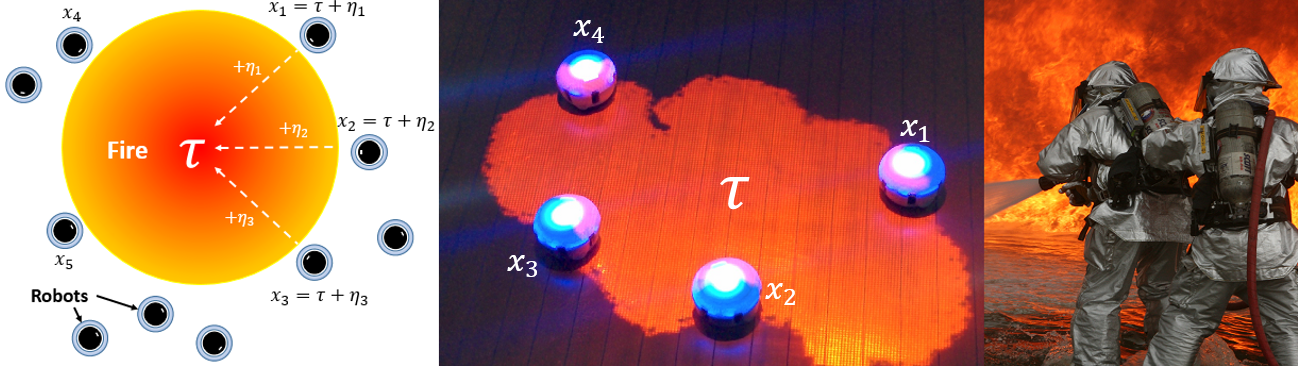
\includegraphics[width=\textwidth]{../figures/dropletfire.png}
\centering\caption{}\label{fig:dropletfire}
\end{figure*}

The goal of this paper is to prove that a response threshold strategy for a broad class of task assignment problems seen in biological and artificial MASs results in unique system-wide equilibrium conditions such that no individual agent will receive a better utility by deviating from their strategy to act based on some threshold value-$k$. 

To prove this statement we employ a sub-class of Game Theory called \emph{global games}, first introduced by Carlsson and Van Damme in 1993 \cite{Carlsson1993}. Global games have been substantially generalized over the years to study and model different economical phenomena such as pricing debt, currency crisis, and bank runs, and we strongly believe they can be further applied to the analysis of task assignment in MASs. See \cite{Morris2000} and the references therein for more details on applications of global games.

Collaborative tasks for MASs can be formally defined as global games with the property of \emph{concurrent benefit}. Informally, concurrent benefit is an attribute of a collaborative task wherein the exact number of agents required to successfully complete the task is unknown and varies over time due to numerous, complex physical parameters. Many collaborative tasks---particularly those seen in biological systems---exhibit the property of concurrent benefit ranging from distributed mapping, surveillance and coordinated defense of enclosed areas like termite mounds and honey bee hives \cite{Breed1990} to collective transport of heavy objects and even containment of oil spills and forest fires. The probability of success depends, non-linearly, on the average number of agents assigned to that task. For example, in a firefighting scenario (see Fig.~\ref{fig:dropletfire}), a single robot trying to contain a large fire will likely be unsuccessful on its own (and will waste fire retardant in trying) but a group of robots within a certain group size range may be able to contain the flames to a reasonable level of success. This measure of success is related non-linearly to the group size, i.e. where 5 or even 10 robots have a negligible effect on containing the fire, perhaps 12 or more very quickly become capable of succeeding in the task. It is for tasks with this common property that we propose our novel task-assignment algorithm.

The rest of the paper is laid out as follows. The next section presents related work in the field of multi-robot task assignment. Section \ref{sec:ggames} provides a brief introduction to the theory of global games and then formally defines the property of concurrent benefit tasks. We then use this definition to prove a theorem stating system level equilibrium conditions and further explain what an equilibrium condition means for a swarm robot system. Section \ref{sec:} Finally, the Discussion and Conclusion sections provide an analysis of the proposed method of task-assignment in a robotic swarm as well as avenues for further study while re-iterating the major contribution of this paper.

\section{Related Work}\label{subsec:rw}
Recruitment of an exact number of robots to a particular task has been extensively studied using the ``Stick Pulling'' experiment \cite{Lerman2001,Martinoli2004}. The problem of distributing a swarm of robots across a discrete number of sites/tasks with a specific desired distribution has been studied in \cite{Berman2009,Correll2008}. The proposed algorithm extends upon the first group of work, and we show how the proposed stochastic task assignment algorithm reduces to the ones described in \cite{Lerman2001,Martinoli2004} when using appropriate parameters.  Mather \cite{Mather2010} instead presents a stochastic approach that is a hybrid between the work in \cite{Berman2009} and \cite{Martinoli2004}, allowing assignment to tasks requiring a varying number of robots.
While a response threshold function can also be applied to the swarm distribution problem, this problem is complementary to the problem of recruiting teams of varying sizes addressed in this paper. 

We also prove that using an agent based threshold policy for task assignment results in an equilibrium for the whole swarm system using the theory of global games So far as we are aware, global games have never been used in the context of swarm robotics before and this is a novel approach to proving system-level equilibrium, i.e. no individual agent can perform better by deviating from a threshold based policy.

\section{Global Games: A Brief Overview}\label{sec:ggoverview}
Game theory is the study of strategic interactions among multiple agents or players, such as robots, people, firms, etc. where the decision of each party affects the payoff of the rest. A fundamentally important class of games is one with incomplete information where each agent's utility depends not only on the actions of the other agents but also on an underlying fundamental signal that cannot be accurately ordained by the agents. Returning to our previous example of firefighting, this fundamental signal is the difficulty of the task of putting out the fire. The size and intensity of the fire, along with environmental and other site-specific factors all play a major role in determining whether an agent should begin the task or wait for more help to arrive. 

This class of global games with incomplete information was originally introduced in \cite{Carlsson1993} where two players are playing a game and the utility of the two players depends on an underlying fundamental signal-$\tau$ but each agent observes a noisy variation of this signal, $\estt_i$. Note that noisy variation in $\tau$ is not a result of inaccuracy in sensor measurements but represents a culmination of underlying unknown factors of the scenario. We discuss how sensor noise, from agents measuring the fundamental signal, can be modeled in the following section.

\section{Situating Global Game Theory in a Multi-Agent System Setting}\label{sec:ggmas}



\section{Concurrent Benefit Task with Incomplete Information}\label{sec:conbenefit}
In this section, we mathematically define a concurrent benefit task which is central to our study. Consider a set of $n$ robots and suppose that each robot has an action set $A_i=\{0,1\}$ where $0$ represents ``not participating'' in the task and $1$ represents ``participating'' in the task.  Another object which plays an important role in our formalism is the \textit{easiness} parameter $\tau$ of the given task. We let $\tau$ be an (often random) real number which simply represents how easy/hard a task is and we further assume that it belongs to an interval $E=[c,d]$ in $\R$.  Finally, we let $u_i:A_1\times\Z^+\times \R\to \R$ be the utility of the $i^{\text{th}}$ robot, where $u_i(a_i,g,\tau)$ is the utility of the $i^{\text{th}}$ robot when $g$ other robots have decided to participate in the task and $\tau$ is the easiness parameter of the task\footnote{In general, the utility of each robot depends on the joint actions of the rest of the robots. However, here we assume that the utility depends only on the number of robots participating in the activity. The following discussions can be substantially generalized to a more general setting but this form of utility serves the purpose of this study.}. 

\begin{figure}[!htb]
\centering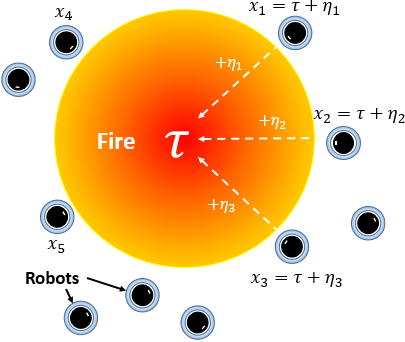
\includegraphics[width=.75\columnwidth]{../figures/globalgamesetup.png}
\centering\caption{}\label{fig:ggsetup}
\end{figure}

We define a task $T$ to be a \textit{concurrent benefit task} if: 
\begin{enumerate}[a.]
	\item $u_i(1,g,\tau)\geq u_i(0,g,\tau)$ for all $g\in[n-1]:=\{0,1,\ldots,n-1\}$ and $\tau \in E$. 
	\item $u_i(a_i,g,\tau)$ is an increasing and continuous function of $\tau$ for any $a_i$ and $g$. 
	\item $u_i(1,g,\tau)-u_i(0,g,\tau)\geq u_i(1,g',\tau)-u_i(0,g',\tau)$ for any $g\geq g'$ in $[n-1]$ and any $\tau\in E$. In other words, the more the number of the rest of the robots participating in the task, the more beneficial would be taking part in the activity.
	\item For any $g$ and any $\tau\geq \tau'$, we have $u_i(1,g,\tau)-u_i(0,g,\tau)\geq \lambda (\tau-\tau')$. 
	\item For extreme easiness factors, taking part in the activity has unique trivial equilibrium, i.e. there exists $\underline{\tau},\bar{\tau}\in (c,d)$ with $\underline{\tau}\leq \bar{\tau}$ such that for any $\tau\geq \bar{\tau}$, the only equilibrium of the game is $(1,1,\ldots,1)$ and for $\tau\leq \underline{\tau}$, the only equilibrium of the game is $(0,0,\ldots,0)$.
\end{enumerate}

Note that in order to have such a task, we need the above conditions to hold for all the robots, i.e. for all $i\in\{1,\ldots,n\}$.
An example of a utility function that would satisfy such conditions is a function $u_i(a_i,g,\tau)=a_i(\beta_is+\gamma_i\tau)$ with $\beta_i,\gamma_i\geq 0$, and $c<0$.

The main challenge in devising strategies in performing a concurrent benefit task is that the knowledge of the easiness parameter is not easily accessible to the robots. For example consider the firefighting task described above. In this task, how easy/hard the task is not exactly clear for each robot. Rather, each robot, with the help of the sensors on board, has some knowledge of this factor. We model this imperfect knowledge by assuming that robot $i$ observes $x_i=\tau+\nu \eta_i$ where $\eta_i$ is a continuous random variable with finite support and $\nu\geq 0$ is a parameter of the system. 

\section{Theorem and Proof}\label{sec:thmproof}
Given the above scenario, we say that $s_i:\R\to \{0,1\}$ is a pure strategy if  $s_i$ maps any private measurement $x_i$ to an action in $\{0,1\}$. We say that $s_i$ is a threshold strategy if there exists some $\tau$ such that $s_i(x_i)=1$ for $x_i\geq \tau$ and $s_i(x_i)=0$ if $x_i<\tau$. In other words, $s_i$ prescribes taking part in the task if the private information is small and prescribes not taking part in the activity if the private measurement is large. 

\begin{theorem}
Let task $T$ be a task satisfying the above conditions and suppose that the easiness factor $\tau$ is uniformly distributed over $E$. Then, for sufficiently small $\nu>0$, there exists a unique joint strategy $s^*=(s_1^*,s_2^*,\ldots,s_n^*)$ that survives iterative strict dominance. Moreover, the strategy $s^*$ is a threshold equilibrium, i.e.\ each $s_i^*$ is a threshold strategy.
\end{theorem}

\begin{proof}
\textbf{To be done by Behrouz\ldots}
\end{proof}



\section{Discussion}\label{sec:disc}




\section{Conclusion}\label{sec:conc}




%%%%%%%%%%%%%%%%%%%%%%%%%%%%%%%%%%%%%%%%%%%%%%%%%%%%%%%%%%%%%%%%%%%%%%%%%%%%%%%%
%%%%%%%%%   The Bibliography, if any   %%%%%%%%%
\bibliographystyle{IEEEtran}		% or "siam", or "alpha", etc.
\nocite{*}
\bibliography{../refworks}
\end{document}
